\documentclass{acm_proc_article-sp}

\usepackage{listings}
\usepackage{float}

\floatstyle{plain}
\newfloat{program}{thp}{lop}
\floatname{program}{Query}

\begin{document}
\lstset{language=SQL}


\title{Inner Workings Behind Babel
}
\subtitle{[Conversion Specifications]}

\numberofauthors{3} 
\author{
% 1st. author
\alignauthor
Frank Roetker
       \affaddr{Rose-Hulman Institute of Technology}\\
       \affaddr{5500 Wabash Ave.}\\
       \affaddr{Terre Haute, IN, USA}\\
       \email{roetkefj@rose-hulman.edu}
% 2nd. author
\alignauthor
Jordon Phillips
       \affaddr{Rose-Hulman Institute of Technology}\\
       \affaddr{5500 Wabash Ave.}\\
       \affaddr{Terre Haute, IN, USA}\\
       \email{phillijk@rose-hulman.edu}
% 3rd. author
\alignauthor Ricky Shomer
       \affaddr{Rose-Hulman Institute of Technology}\\
       \affaddr{5500 Wabash Ave.}\\
       \affaddr{Terre Haute, IN, USA}\\
       \email{shomerrt@rose-hulman.edu}
}
\date{15 May 2013}

\maketitle
\begin{abstract}
In the world of database management systems, relational databases are dominate. This isn't too surprising since a relational database can be used to solve many problems. However, using a relational database as a solution is not always the most efficient answer.

Babel seeks to alleviate the problem of a company being locked-in to using a RDBMS. A company isn't going to throw away their data stored in a RDBMS to restart with a graph database even if it might speed up their query times. However, if given a tool that was to fully export their data to a Neo4j system, they might. 
\end{abstract}

% A category with the (minimum) three required fields
% \category{H.4}{Information Systems Applications}{Miscellaneous}
%A category including the fourth, optional field follows...
% \category{D.2.8}{Software Engineering}{Metrics}[complexity measures, performance measures]

% \terms{}

\keywords{Neo4j, Cypher}

\section{Introduction}

In the world of database management systems, relational databases are dominate. This isn't too surprising since a relational database can be used to solve many problems. However, using a relational database as a solution is not always the most efficient answer.

NoSQL has gained a footing in the database domain, solving problems in a different light than Relational databases. Neo4j, a NoSQL graph database takes a much different stance when viewing the world. ``Reality is a graph''\cite{neo4j:neo4j} is the mantra that Neo Technology takes when looking at data. This may be a greater fit for solving problems that involve deeply connected data which in a RDBMS would be distributed across many tables and relying on many foreign keys. \cite{webber:graph}

Babel seeks to alleviate the problem of a company being locked-in to using a RDBMS. A company isn't going to throw away their data stored in a RDBMS to restart with a graph database even if it might speed up their query times. However, if given a tool that was to fully export their data to a Neo4j system, they might.

\section{Babel}

Babel seeks to be the tool to solve that problem. Given connection strings to both databases, it queries information from the SQL database, analyzes it, and creates an equivalent Neo4j database. Using the labels feature found in the most recent versions of Neo4j it can even create eqivalent indicies, allowing for fast and simple queries.

\subsection{MS SQL data}

The first step in the process of converting a MS SQL database to another database is defining the SQL queries to find all correct data from the MS SQL database. This is actually not as much of an issue; MS SQL Server keeps much of this data for you.

In a relational database, foreign key tables are commonly used to join
multiple tables together. This is the equivalent to relationships in
our graph database. So our query needs to include foreign keys, their tables, and the tables/columns that they are constrained to:

\begin{program}
\begin{lstlisting}[frame=single,breaklines=true]
SELECT INFO.TABLE_NAME, INFO.COLUMN_NAME, 
       FK.FKTABLE_NAME, FK.FKCOLUMN_NAME 
FROM

(SELECT TABLE_NAME, COLUMN_NAME
        FROM INFORMATION_SCHEMA.COLUMNS) AS INFO

LEFT OUTER JOIN

(
 SELECT C.TABLE_NAME [TABLE_NAME], 
        KCU.COLUMN_NAME [COLUMN_NAME],
        C2.TABLE_NAME [FKTABLE_NAME], 
        KCU2.COLUMN_NAME [FKCOLUMN_NAME]
  FROM  INFORMATION_SCHEMA.TABLE_CONSTRAINTS C 
        INNER JOIN INFORMATION_SCHEMA.KEY_COLUMN_USAGE KCU 
          ON C.CONSTRAINT_SCHEMA = KCU.CONSTRAINT_SCHEMA 
            AND C.CONSTRAINT_NAME = KCU.CONSTRAINT_NAME 
        INNER JOIN INFORMATION_SCHEMA.REFERENTIAL_CONSTRAINTS RC 
          ON C.CONSTRAINT_SCHEMA = RC.CONSTRAINT_SCHEMA 
            AND C.CONSTRAINT_NAME = RC.CONSTRAINT_NAME 
        INNER JOIN INFORMATION_SCHEMA.TABLE_CONSTRAINTS C2 
          ON RC.UNIQUE_CONSTRAINT_SCHEMA = C2.CONSTRAINT_SCHEMA 
            AND RC.UNIQUE_CONSTRAINT_NAME = C2.CONSTRAINT_NAME 
        INNER JOIN INFORMATION_SCHEMA.KEY_COLUMN_USAGE KCU2 
          ON C2.CONSTRAINT_SCHEMA = KCU2.CONSTRAINT_SCHEMA 
            AND C2.CONSTRAINT_NAME = KCU2.CONSTRAINT_NAME 
            AND KCU.ORDINAL_POSITION = KCU2.ORDINAL_POSITION 
 WHERE  C.CONSTRAINT_TYPE = 'FOREIGN KEY'
) AS FK

ON FK.TABLE_NAME = INFO.TABLE_NAME
   AND FK.COLUMN_NAME = INFO.COLUMN_NAME
ORDER BY INFO.TABLE_NAME, INFO.COLUMN_NAME
\end{lstlisting}
\caption{SQL Table Data}
\end{program}

This consolidation of data is what we are going to need to consider when
designing the algorithm for distinguishing potential nodes from relationships.

\subsection{Conversions}

This section will explain how Tables are going to be converted for 
Neo4j\footnote{These are ordered in order of complexity, not number of
Foreign keys}.

In the Relational database world, data is organized in Tables (or Relations). These tables are made up of Columns (\textit{Attributes}) and Rows (or Tuples). There is also the notion of Foreign keys. These allow data from one table to be consistent with data from another - allowing the data in tables to be joined.

Graph databases on the other hand join data in a much more organic way. The idea of Tuples is thrown out for Nodes. These nodes have Properties; properties are similar to columns. As for the graph relative to Foreign keys, we have Relationships. However, Relationships are much more than just a Foreign key: they physically connect Nodes to each other. Like Nodes, Relationships also can also have properties.

\begin{figure*}
  \centering
  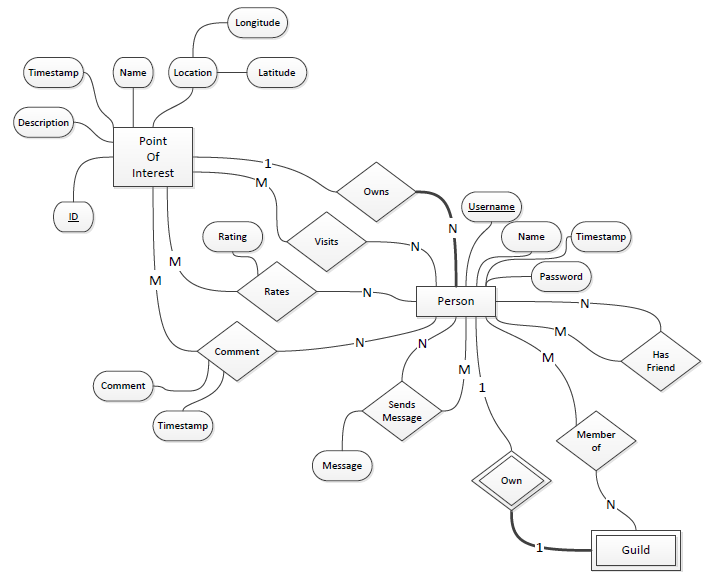
\includegraphics[width=0.75\textwidth]{Images/URBEX_ERD}
  \caption{Urban Exploration Entity Relationship Diagram}
\end{figure*}

\subsubsection{0 Foreign Keys}

In the event that the table in question has 0 foreign keys, we would consider it a ``Base Table''. This table does not rely on any other information stored in any other table and thus is an entity in and of itself.

We treat tuples from this type of table as a Node in regards to Neo4j. This is the simplest conversion between MS SQL and Neo4j, because it doesn't rely on any other data already existing in the database. This conversion will make a new node with Properties for each Attribute owned by the Tuple.

\subsubsection{2 Foreign Keys}

The next table conversion to understand is the conversion for the 2 foreign key tables. These tables are usually called ``Foreign Key Tables'' because they are usually devoted to easily joining two tables.

Since we have defined basic tables as Nodes in Neo4j, we could say that these foreign key tables are joining these two tables. In the graph database world, this joining of tables is a Relationship. This conversion will make a new relationship between two nodes and give this relationship Properties for each Attribute owned by the Tuple in the given foreign key table.

\subsubsection{1 Foreign Key}

Now we are getting into the more diverse types of conversions that Babel performs. \footnote{There are multiple approaches to converting tables that are neither of the two previously explained tables, and it is not the goal of this paper to convince you that Babel's approach is the best.} These conversions are a mixture of the two previous forms and are actually quite simple when taking a closer look at the data.

Tables that have 1 foreign key don't fit the mold of either of the two previously described conversions. They can't simply be a Node because there is obviously a piece of their data that is connected to some other tuple, but they also can't simply be a Relationship because they don't connect two tables. 

However, we can take those two principles and merge them together. The simple data that describes them as a Node does exactly that. Then the foreign key will be used as a Relationship between this node created and some other node that the data is referring to.

\subsubsection{3 Or More Foreign Keys}

Things brings us to how we handle tables that have 3 or more foreign keys. Well Babel handles these tables are the same way that it handles tables with 1 foreign key: it creates a Node with many Relationships\footnote{It creates as many Relationships as there are foreign keys.}.

\subsection{Conversion Example}

In this guide, I will be using an Urban Exploration database as an example. You don't need to have an understanding of what the database will represent or what the data means to understand how the conversions are going to be handled. Please refer to Figure 1 for the Entity Relationship Diagram for the database in this example.

After running our SQL query on the database, we will be presented with the results that are in Figure 2. After viewing these results, it may become more clear how the data is going to be divided up.

Determing how to create the Neo4j database based off the query in Figure 2, we must look at how many foreign keys each table contains.  Using the foreign key cases descriped above, we can determine that the Comment table will become a relation with attributes Comment and TimeStamp, and will be pointing to the nodes Point of Interest and Person.  The Friend table will became a relation with no attributes connected to two seperate Person nodes.  The Guild table will become a node containing the attributes Description, Name, and PUsername. 

Additionally, the Membership table will form a relationship connecting the Guild and Person nodes.  The Owns table will form a relation which related the Point of Interest node and the Person node.  Also, the Person table will become a node containing the attributed Name, Password, TimeStamp, and username. 

Continuing with this trend, the Point of Interest table will form a node which contains the Code, Description, id, Latitude, Longitude, Name, and TimeStamp attributes.  The Rate table will form yet another relation which has the Rating attribute and connects the Person and Point of Interest nodes.  Lastly, the Visit table with form the final relation which again connects the Point of Interest and Person nodes.  After all is complete, we have just created the Neo4j equivalent database to the one display in Figure 1. 

\begin{figure}
  \caption{Table Info from Query 1}
  \centering
    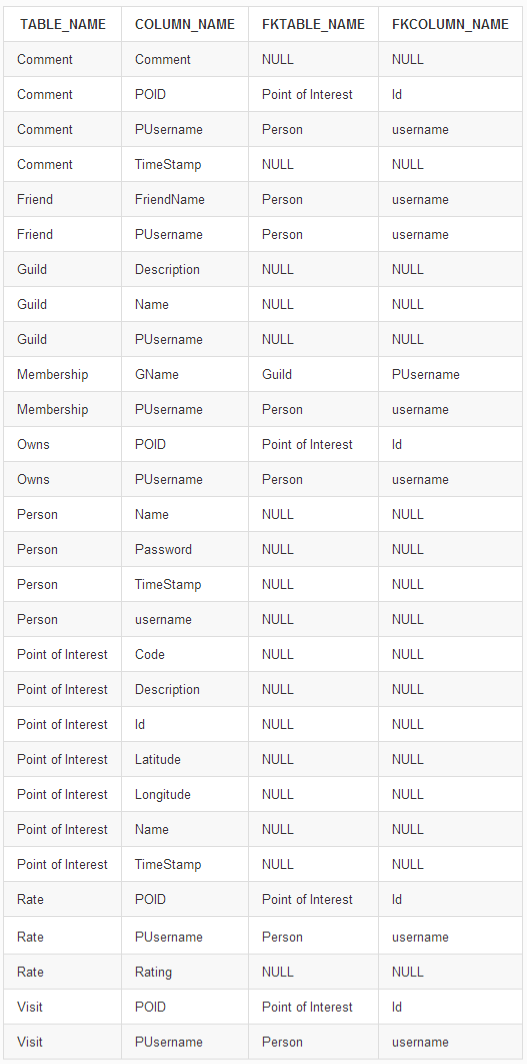
\includegraphics[width=0.45\textwidth]{Images/TableInfo}
\end{figure}

\section{Conclusions}

Babel was created to aid in the transition from a typical RDBMS to a graph database format.  It allows companies to follow their innovative inspirations, and break stereotypical trends.  The accomplishment of Babel was not necessarily the code produced for the application, but perhaps the though process behind converting a relational database to a graph database.  Babel covers all ends of the spectrum and successfully manages to convert cases close to the extrema.


\subsection{Future Additions}

Babel has a number of additions planned for the future. Babel, being written for Neo4j v2.0.0-M02, makes use of the new features in store for the next release of Neo4j. These features are not all fully developed, and thus Babel is limited in many ways.

First, the Rest API that is provided for Neo4j has the option for nodes to be inserted in a bulk transaction. This greatly increases the speed of inserts, because one transaction is much faster than having to wait for as many transactions as there are tuples. Babel does not currently use this option, due to the fact that nodes do not yet have the ability to gain a label in the Rest API for bulk inserts.

Relationships are expensive actions. Babel currently queries the nodes added to the database for their address before creating a relationship between them. This would mean that relationships take at most 3 transactions before they are created. The most obvious option to move forward from where we are right now would be to cache the location of the nodes after inserting them into Neo4j. This would reduce relationship creation to one transaction. From there, we could even use a bulk insert for relationships, reducing their transaction count to even less.

Another plan that is in store for Babel is continuous updates from the MS SQL Server. Babel currently only supports running once per Neo4j database; if you want to update a Neo4j database with new information that was added to MS SQL Server, you will need to purge the database and then rerun Babel. Forgoing this issue and allowing users to run Babel as many times as they want without having to purge their databases is of great importance.

%ACKNOWLEDGMENTS are optional
\section{Acknowledgments}

We would like to thank Dr. Sriram Mohan for his help during the start of this project. Without his guidance, we would not have achieved our final product.

%
% The following two commands are all you need in the
% initial runs of your .tex file to
% produce the bibliography for the citations in your paper.
\bibliographystyle{abbrv}
\bibliography{MSSQL-Neo4j}  % MSSQL-Neo4j.bib is the name of the Bibliography in this case
% You must have a proper ".bib" file
%  and remember to run:
% latex bibtex latex latex
% to resolve all references
%
% That's all folks!
\end{document}
